\documentclass[
  bibliography=totoc,     % Literatur im Inhaltsverzeichnis
  captions=tableheading,  % Tabellenüberschriften
  titlepage=firstiscover, % Titelseite ist Deckblatt
]{scrartcl}
\usepackage{scrhack}
\usepackage[aux]{rerunfilecheck}
\usepackage{fontspec}
\usepackage[ngerman]{babel}
\usepackage{graphicx}
\usepackage[section, below]{placeins}
\usepackage{caption}
\usepackage{scrlayer-scrpage}
%Mathe Pakete
\usepackage{amsmath}
\usepackage{amssymb}
\usepackage{mathtools}
\usepackage{xfrac}
\usepackage[math-style=ISO,bold-style=ISO,sans-style=italic,nabla=upright,partial=upright]{unicode-math}
\usepackage[
  math-style=ISO,
  bold-style=ISO,
  sans-style=italic,
  nabla=upright,
  partial=upright,
]{unicode-math}
\usepackage[
  locale=DE,
  separate-uncertainty=true,
  per-mode=symbol-or-fraction,
]{siunitx}
\usepackage{subcaption}
\usepackage{graphicx}
\usepackage{booktabs}
\usepackage{microtype}
\usepackage[unicode]{hyperref}
\usepackage{bookmark}
\setmathfont{Latin Modern Math}
\usepackage{csquotes}
\usepackage{wrapfig}
\usepackage[shortcuts]{extdash} % Trennung von Wörtern mit Strichen
\usepackage[backend=biber]{biblatex} %Literaturverzeichnis
\addbibresource{lit.bib}
\usepackage[section]{placeins}%Floats plazieren
\usepackage[version=4, math-greek=default,text-greek=default,]{mhchem} %Chemische Zeichen

\begin{document}
  \setlength{\parindent}{0em} %keine Einrückungen am Zeilenanfang
  \pagestyle{scrheadings}
  \clearpairofpagestyles
  \ofoot{\pagemark}

  \title{V 354 \\ Gedämpfte und erzwungene Schwingungen}
  \author{Julian Hayduk \and Alex Nuss}
  \date{Durchführung: 06.12.2022, Abgabe: 13.12.2022}
  \subtitle{Versuchsort: TU Dortmund }
  \maketitle

  \thispagestyle{empty}
  \newpage
  
  \tableofcontents
  \thispagestyle{empty}
  \setcounter{page}{1}
  
  \newpage
  \section{Ziel des Versuches}
  
  In diesem Versuch werden der effektive Dämpfungswiderstand, der Dämpfungswiderstand,
  bei dem der aperiodische Grenzfall auftritt sowie die Frequenzabhängigkeit gedämpfter
  und erzwungener Schwingungen bestimmt. Dazu wird ein RLC Schwingkreis
  untersucht.
  
  \section{Theorie}
  
  \label{sec:Theorie}
  \subsection{Gedämpfte Schwingung}
  In \autoref{fig:rlc} ist die prinzipielle Schaltung eines gedämpften Serienschwingkreises dargestellt. 
  \begin{figure}[h]
      \centering
      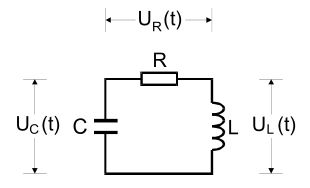
\includegraphics{rlc.JPG}
      \caption{Schaltung eines gedämpften Serienschwingkreises. [1]}
      \label{fig:rlc}
    \end{figure}
  \noindent 
  Durch diese Schaltung wird eine gedämpfte Schwingung der Energie realisiert, die
  zwischen den beiden Speichern (Spule L und Kapazität C) hin und her pendelt. Der
  Widerstand R sorgt für die Dämpfung der Schwingung, indem er elektrische Energie
  irreversibel in Wärmeenergie umwandelt. Für diese Schaltung kann mit dem 2. Kirchhoffschen
  Gesetz eine Differentialgleichung (DGL) ermittelt werden.

  \begin{equation}
      U_{\symup{R}} + U_{\symup{C}} + U_{\symup{L}}   = 0     
      \label{eqn:masche}
  \end{equation}

  \noindent Die Spannungsbeziehungen für die 3 Bauelemente sind durch die Beziehungen
      \begin{align}
          U_{\symup{R}} & = RI \\
          U_{\symup{C}} & = \frac{Q}{C}\\
          U_{\symup{L}} & = L \cdot \symup{\frac{d}{dt}}I 
      \end{align}
  \noindent gegeben. 
  Mit diesen Beziehungen und $I=\symup{\frac{d}{dt}}Q$ kann die DGL für die Schaltung mit einmaligem Ableiten aufgestellt werden:
  \begin{align}
          L  \symup{\frac{d}{dt}}I + RI + \frac{Q}{C} & = 0 \\
        \iff \symup{\frac{d^2}{dt^2}}I + \frac{R}{L} \symup{\frac{d}{dt}}I + \frac{1}{LC}I & = 0 
          \label{eqn:dgl}
  \end{align}
      
  \noindent Die DGL kann mit einem komplexen $\symup{e}$-Funktionsansatz gelöst werden.
      \begin{equation}
          I(t) = A \cdot \symup{e}^{j \tilde{w} t}
          \label{eqn:dgl2}
      \end{equation}

      \begin{equation}
          \tilde{\omega}_{1,2} = j \frac{R}{2L} \pm \sqrt{\frac{1}{LC}-\frac{R^2}{4L}} 
          \label{eqn:dgl3}
      \end{equation}
      
      \noindent Das heißt $I(t)$ lässt sich durch folgende Gleichung ausdrücken:
      \begin{equation}
          I(t) = A_1 \cdot \symup{e}^{j \tilde{w}_1t} + A_2 \cdot \symup{e}^{j\tilde{w}_2 t} 
      \end{equation}

  \noindent Es lassen sich nun 3 unterschiedliche Fälle für die Lösung der DGL, in Abhängigkeit des Wurzelterms in \autoref{eqn:dgl3}, unterscheiden. 
  Im ersten Fall ist $\frac{1}{LC} > \frac{R²}{4L²}$ und die Wurzel in \autoref{eqn:dgl3} bleibt reell. Dieser Fall wird als Schwingfall bezeichnet. Der typische Verlauf der Stromstärke für diesen Fall ist in \autoref{fig:daempf} dargestellt.
  \begin{figure}[h]
      \centering
      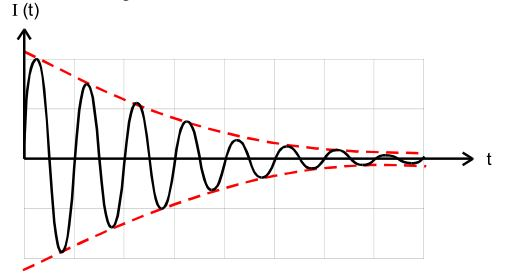
\includegraphics{daempf.jpg}
      \caption{Verlauf der Stromstärke einer gedämpften Schwingung abhängig von der Zeit. [1]}
      \label{fig:daempf}
    \end{figure}
  \noindent
  Die in \autoref{fig:daempf} gestrichelt gezeichnete Einhüllende der Schwingung ist eine e-Funktion der Form
  \begin{equation*}
      \pm U_0 e^{-2\pi\mu t} \\ \text{.}
      \label{eqn:einh}
  \end{equation*}
  \noindent
  Für den zweiten Fall gilt:
  \begin{equation}
      \frac{1}{LC} < \frac{R^2}{4L^2} 
  \end{equation}

  \noindent In diesem Fall ist $\tilde{\omega} \in \mathbb{C}$.
  Den Fall

  \begin{align*}
  \frac{1}{LC} &= \frac{R²}{4L²}\\
  \iff R &= 2\sqrt{\frac{L}{C}}
  \end{align*}

  \noindent bezeichnet man als aperiodischen Grenzfall. In diesem Fall bewegt sich $I(t)$ ohne 
  Überschwingen am schnellsten gegen 0. 
  \subsection{Erzwungene Schwingung}
  Um erzwungene Schwingungen mit einem elektrischen Schwingkreis zu realisieren, kann die Schaltung aus \autoref{fig:rlc} zu der Schaltung aus \autoref{fig:erzwungen} erweitert werden. Hier sorgt eine Spannungsquelle mit sinusförmiger Wechselspannung für die äußere Anregung.
  \begin{figure}[h]
      \centering
      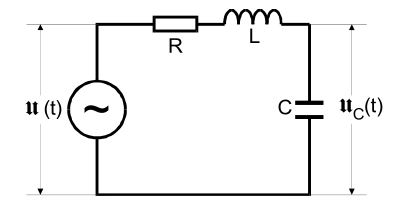
\includegraphics{erzwungen.JPG}
      \caption{Schaltung zur Erzeugung einer erzwungenen Schwingung. [1]}
      \label{fig:erzwungen}
    \end{figure}
  \noindent
  Die DGL dieser Schaltung lässt sich wieder über die Kirchhoffschen Gesetze aufstellen. Mit den bereits beschriebnen Zusammenhängen für die Spannungen an den einzelnen Bauelementen lässt sich die DGL außerdem für die Kondensatorspannung $U_C$ umschreiben:
  \begin{equation}
      LC \frac{\text{d}^2 U_C}{\text{dt}^2} + RC \frac{\text{d} U_C}{\text{dt}} + U_C = U_0 e^{j \omega t}.
  \end{equation}
      
  \noindent Auch diese DGL kann wieder mit einem komplexen $\symup{e}$-Funktionsansatz gelöst werden. Auf diese Weise erhält man für $U_C$:
  \begin{equation}
      U_C(\omega) = \frac{U_0}{\sqrt{(1-LC\omega^2)^2 + \omega^2 R^2 C^2}}.
      \label{eqn:uc}
  \end{equation}
  \noindent Wie an \autoref{eqn:uc} zu sehen ist, strebt $U_C$ für $\omega \to \infty $ gegen 0 und für $\omega \to 0$ gegen die Erregerspannung $U_0$. Außerdem existiert ein $\omega_{\text{res}}$, die sogenannte Resonanzfrequenz, bei der $U_C$ maximal wird. Als Wert für die Resonanzfrequenz kann
  \begin{equation}
      \omega_{\text{res}} = \sqrt{\frac{1}{LC}-\frac{R^2}{2L^2}} 
  \end{equation}
  \noindent berechnet werden. Für den interessanten Fall von schwacher Dämpfung, also für
  \begin{equation*}
      \frac{R^2}{2L^2} << \frac{1}{LC}
  \end{equation*}
  nähert sich $\omega_{\text{res}}$ der Kreisfrequenz $\omega_0=\frac{1}{\sqrt{LC}}$ der ungedämpften Schwingung an. Für diesen Fall ergibt sich für $U_C$:
  \begin{equation}
      U_{\text{C,max}} = \frac{1}{\omega_0 RC} U_0 = \frac{1}{R} \sqrt{\frac{L}{C}} U_0 
      \label{eqn:ucmax}
  \end{equation}
  Wie an \autoref{eqn:ucmax} zu sehen ist, strebt $U_C$ für $R \to 0 $ gegen $\infty$. Dieser Fall wird auch als Resonanzkatastrophe bezeichnet. Der Faktor $\frac{1}{\omega_0 RC}$ ist die sogenannte Resonanzüberhöhung oder Güte q des Schwingkreises.
  \newline
  Die Güte q kann in ein Verhältnis zu der Breite der Resonanzkurve gebracht werden. Die Breite wird dabei über die Frequenzen  $\omega_+$ und $\omega_-$ charakterisiert, bei denen $U_C$ auf einen Anteil von $\frac{1}{\sqrt{2}}$ von ihrem Ursprungswert abgefallen ist. Mit \autoref{eqn:uc} und \autoref{eqn:ucmax} lässt sich dies als
  \begin{equation}
      \frac{U_0}{\sqrt{2}} \frac{1}{\omega_0 RC} = \frac{U_0}{C \sqrt{\omega^2_{\pm} R^2 + ( \omega^2_{\pm}L - \frac{1}{C} ) }}
  \end{equation} 
  schreiben. Mit der Breite der Resonanzkurve
  \begin{equation}
      \omega_+ - \omega_- \approx \frac{R}{L}.
      \label{eqn:breite}
  \end{equation}
  ergibt sich dann als Zusammenhang von Güte und Breite:
  \begin{equation}
      q = \frac{\omega_0}{\omega_+ - \omega_-}
      \label{eqn:guete}
  \end{equation}
  
  
  \section{Fehler}
  \label{sec:Fehler}
  Der Mittelwert:
  \begin{center}
    \begin{equation}
      \label{eq:Mittelwert}
    \bar{x} = \frac{1}{n} \sum \nolimits_{i=0} x_i
    \end{equation} 
  \end{center}

  Die Standardabweichung:
  \begin{center}
    \begin{equation}
      \label{eq:standardabweichung}
      \sigma=\sqrt{\frac{\sum(x_i-\bar{x})^2}{n-1}}
    \end{equation}
  \end{center}

  Der Fehler des Mittelwertes:
  \begin{center}
    \begin{equation}
      \label{eq:mittelwertfehler}
      \sigma_{\bar{x}}=\frac{\sigma}{\sqrt{n}}
    \end{equation}

    
  \end{center}

  Die Gaußsche Fehlerfortpflanzung:
  \begin{center}
  \begin{equation}
    \label{eq:gaussfehler}  
  \sigma_x=\sqrt{(\frac{\partial f}{\partial x_1})^2\sigma_{x_1}^2+(\frac{\partial f}{\partial x_2})^2\sigma_{x_2}^2+...+(\frac{\partial f}{\partial x_n})^2\sigma_{x_n}^2}
  \end{equation}
  \end{center}

  Die Prozentuale Abweichung:

  \begin{center}
    \begin{equation}
      \label{eq:prozentuale} 
      Abweichung=\frac{ExperimentellerWert - Theoriewert}{Theoriewert}\times 100 
    \end{equation}
    \end{center}
  
  
  \newpage
  \section{Durchführung}
  \label{sec:Durchführung}
  \subsection{Aufbau}
  Um die Zielsetzung des Versuchs zu erreichen, werden die 3 in \autoref{fig:aufbaua}, \autoref{fig:aufbaub} und \autoref{fig:aufbauc} zu sehenden Schaltungen aufgebaut.
  \begin{figure}[h]
      \centering
      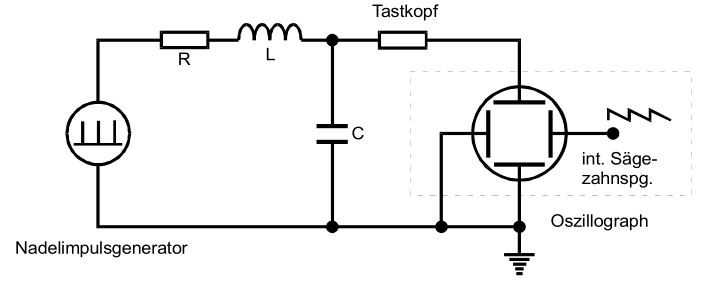
\includegraphics[width=\textwidth]{aufbaua.JPG}
      \caption{Schaltung zur Messung der Zeitabhängigkeit der Amplitude der gedämpften Schwingung. [1]}
      \label{fig:aufbaua}
    \end{figure}
  \noindent

  \begin{figure}[h]
      \centering
      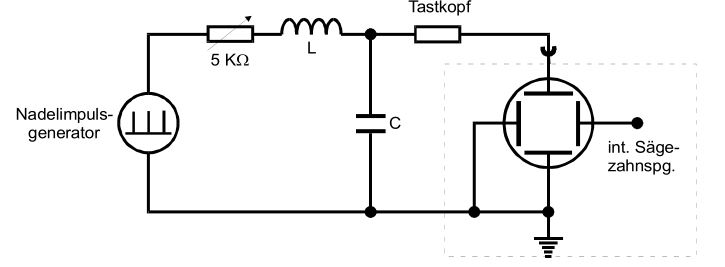
\includegraphics[width=\textwidth]{aufbaub.JPG}
      \caption{Schaltung zur Messung des aperiodischen Grenzwiderstandes $R_{\text{ap}}$. [1]}
      \label{fig:aufbaub}
    \end{figure}
  \noindent

  \begin{figure}[h]
      \centering
      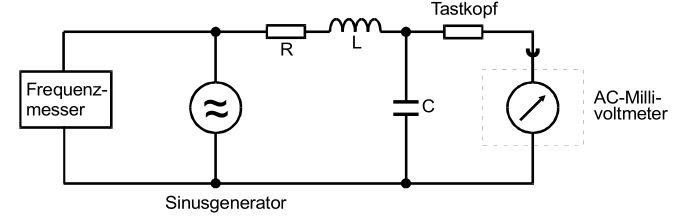
\includegraphics[width=\textwidth]{aufbauc.JPG}
      \caption{Schaltung zur Messung der Frequenzabhängigkeit der Kondensatorspannung eines RLC-Kreises. [1]}
      \label{fig:aufbauc}
    \end{figure}
  \noindent
 
   \subsection{Vorgehensweise}
  Zur Bestimmung der Zeitabhängigkeit der Spannungsamplitude wird die Schaltung aus
  \autoref{fig:aufbaua} genutzt und durch die Apparatur aus \autoref{fig:schaltung}
  realisiert. So werden am Oszilloskop möglichst viele Messwerte für die Spannungsamplitude
  in Abhängigkeit von der Zeit abgelesen. 
  \newline
  Für die Bestimmung des Widerstands
  $R_{\text{ap}}$, bei dem der aperiodische Grenzfall auftritt, wird 
  die Schaltung aus \autoref{fig:aufbaub} verwendet. Dabei wird der regelbare Widerstand an
  der Schaltapparatur genutzt. Nun wird der regelbare Widerstand von seinem Maximalwert
  langsam runter geregelt bis am Oszilloskop zu sehen ist, dass die Kurve kurz vor dem
  Überschwingen ist. Der dann erreichte Widerstand wird notiert.
  \newline 
  Um die Frequenzabhängigkeit der Kondensatorspannung zu
  untersuchen, wird die in \autoref{fig:aufbauc} zu sehende Schaltung verwendet. An dieser
  Schaltung wird dann die Frequenz in einem Bereich von 20 bis 45 kHz variiert. Dabei ist es wichtig
  neben der Frequenz und der entsprechenden Kondensatorspannung auch die Eingangsspannung
  des Generators in Abhängigkeit von der Frequenz zu notieren.
  
  \newpage
  \section{Auswertung}

  \label{sec:Auswertung}

  In diesem Kapitel sollen die aufgenommenen Messwerte ausgewertet werden.
  Über die Schaltung wurden zudem noch folgende Werte notiert:
  \begin{center}
      $L = 10.11 +/- 0.03 \si[]{mH}$,\\
      $C = 2.095 +/- 0.003 \si[]{nF}$,\\
      $R = 48.1 +/- 0.1 {\Omega}$.\\
  \end{center}
  \subsection{Berechnung der Abklingdauer}

  \label{sec:abklingdauer}
  Die aufgenommenen Wertepaare aus Spannung $U(t)$ und $t$ wurden in \autoref{tab:tab2} und \autoref{fig:bild1}
  aufgetragen und es wurde eine Ausgleichskurve hindurchgelegt. Sie hat die Parameter:
  \begin{center}
      
          $a = 3.3568 \pm 0.0669 \Leftrightarrow U_0 = 3.3568 \pm 0.0669 \si{\volt}$ \\
          $b = -1119.1751 \pm 100.4186 \Leftrightarrow \mu = 178.1222 \pm 15.982 \si{\second}$ .\\
      
  \end{center}  
  Der erste Parameter kann hier als Spannung $a=U_0$ interpretiert werden.
  Über die Beziehung 
  \begin{center}
      $R_{eff} = 4\pi\mu L = -2 L b$
  \end{center}


  lässt sich der Dämpfungswiderstand $R_{eff}$, mit $L = 10.11 \pm 0.03 \si{mH}$ zu
  \begin{center}
      $R_{eff} = 22,6 \pm 3.4 \si{\ohm}$
  \end{center}
  bestimmen. Damit lässt sich über \autoref{eq:prozentuale} die prozentuale Abweichung des gemessenen
  gegenüer des Verbauten Widerstandes $R = 48.1 \pm 0.1  {\Omega}$ zu $53\pm 5 \si{\percent}$ bestimmen.
  Nun kann auch die Abklingdauer mithilfe des Zusammenhangs
  \begin{center}
      $T_{ex} = - \frac{1}{b}$
  \end{center}
  berechnet werden. Damit folgt sofort:
  \begin{center}
      $T_{ex} = 0.00089\pm 0.00008 \si[]{s}$. \\
  \end{center}

  \begin{figure}[h]
      \centering
      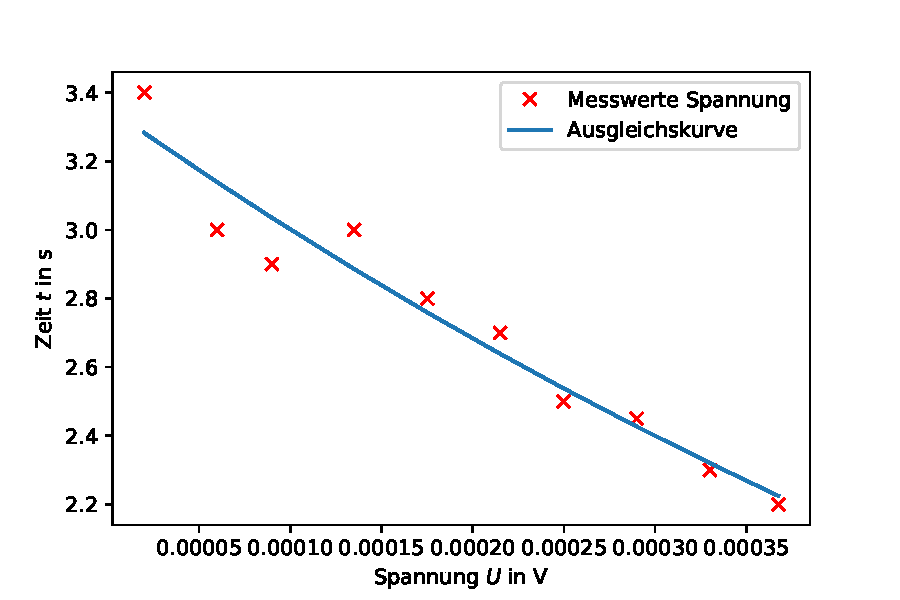
\includegraphics{spannungsverlauf.pdf}
      \caption{Spannungsverlauf in der Zeit}
      \label{fig:bild1}
  \end{figure}

  \FloatBarrier

  \begin{table}[h]
    \centering
    \caption{Messdaten für den Spannungsverlauf}
    \label{tab:tab2}
    \begin{tabular}{c c}
      \toprule
      $t / \si{\micro\second}$ & $U / \si{\volt}$ \\
      \midrule
      20 & 34\\
      60 & 30\\
      90 & 29\\
      135 & 29\\
      175 & 28\\
      215 & 27\\
      240 & 25\\
      270 & 24.5\\
      290 & 23\\
      310 & 22\\
      \bottomrule
    \end{tabular}
  \end{table}
  \FloatBarrier

    \subsection{Der Aperiodische Grezfall}
    \label{sec:apg}
    Der Widerstand wurde solange verändert bis der Aperiodische Grenzfall eingetreten ist. Der zu diesem 
    Zeitpunkt eingestellte Widerstand lag bei:
    \begin{center}
        $R_{ap}=\SI[]{3.02}[]{k\Omega}$.\\
    \end{center}
    Der entsprechende Widerstand lässt sich mit den gegebenen Werten für $L$ und $c$ auch über:
    \begin{center}
        $R_{ap}=2\sqrt{\frac{L}{C}}=4.39+/-0.017\si[]{k\Omega}$
    \end{center}
    bestimmen. Die über \autoref{eq:prozentuale} berechnete prozentuale Abweichung beträgt dann 31,2\%. 

    \subsection{Resonanzüberhöhung}
    \label{sec:res}
    In \autoref{fig:resonanz} ist die Erregerfrequenz gegen die Spannung halblogaritmisch aufgetragen.
    Die rote Linie zeigt dabei an, wo die Resonanzüberhöhung berechnet wurde. In
    \autoref{fig:resonanzzoom} ist nur der Bereich der Resonanzüberhöhung linear dargestellt. Da es keine
    Messwerte gibt welche genau den Wert $\frac{max(U_C)}{U_E*\sqrt{2}}$ mit $U_E=50V$ haben, wurde zwischen
    dem jeweils darüber und darunter liegenden Messwert linear interpoliert. Dies führt zu folgenden Ergebnissen:
    \begin{center}
        $\omega_-=\SI[]{25.2245}[]{\kilo\hertz}$,\\
        $\omega_+=\SI[]{26.6224}[]{\kilo\hertz}$.\\
    \end{center}
    Die Güte lässt sich dann einfach über:
    \begin{center}
        $q=\frac{\omega_0}{\omega_+-\omega_-}$,\\
        $\omega_0=\frac{1}{\sqrt{LC}}$,\\
        $\Rightarrow$ $q=\frac{1}{\sqrt{LC}(\omega_+-\omega_-)} =155.1 \pm 0.4$
    \end{center} 

    Der theoretische Wert lässt sich dann über:
    \begin{center}
        $q=\frac{L}{\sqrt{LC}R}$,\\
        $\Rightarrow$  $q= 45.63\pm 0.18$\\
    \end{center}
    berechnen. Die über \autoref{eq:prozentuale} berechnete prozentuale Abweichung beträgt dann 182.5\%.
    \begin{figure}
      \centering
      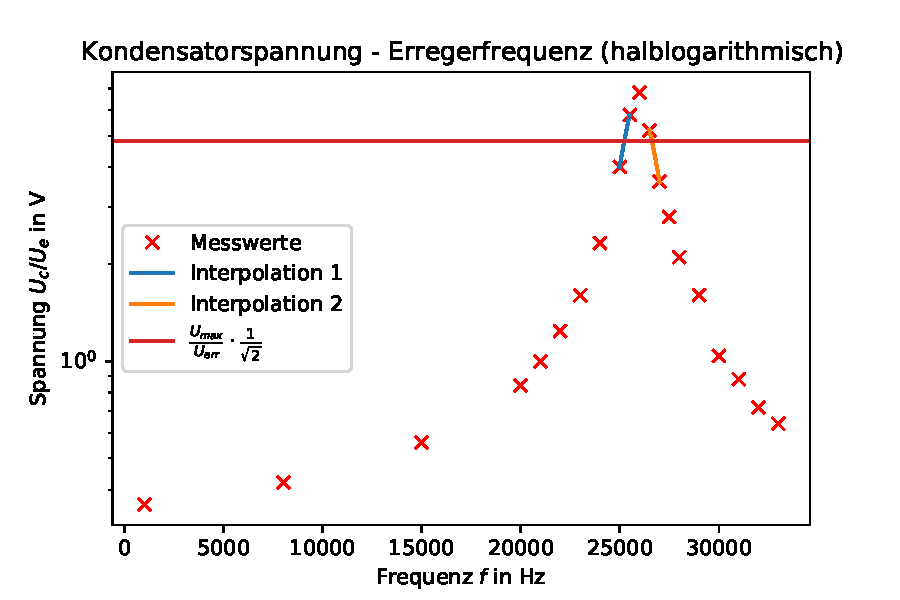
\includegraphics{frequenz.pdf}
      \caption{Spannungsverlauf in Abhängigkeit der Frequenz}
      \label{fig:resonanz}
    \end{figure}

    \begin{figure}
      \centering
      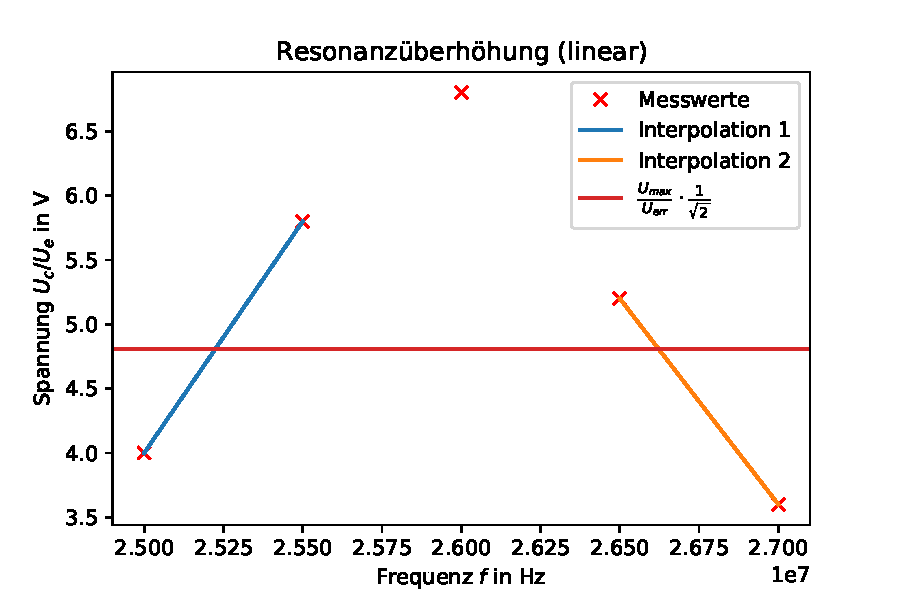
\includegraphics{resonanzuberhohung.pdf}
      \caption{Spannungsverlauf in Abhängigkeit der Frequenz}
      \label{fig:resonanzzoom}
    \end{figure}

  \subsection{Phasenverschiebung}
  \label{sec:phs}
  Aus der als Zeitwerte gemessenen Phasenverschiebung lassen sich über:
  \begin{center}
      $\phi=\Delta tf360°$\\
  \end{center}
  die Phasenverschiebungen in Grad berechnen. Sie wurden in \autoref{fig:phasenverschiebung} halblogaritmisch gegen die Frequenz
  aufgetragen. In \autoref{fig:phasenverschiebung2} sind dieselben Werte noch einmal linear aufgetragen. Zudem
  sind hier noch Graden bei den Winkeln 45°,90° und 135° eingetragen. Um die zugehörigen Frequenzen zu finden wurde
  wieder linear interpoliert.
  \begin{figure}
      \centering
      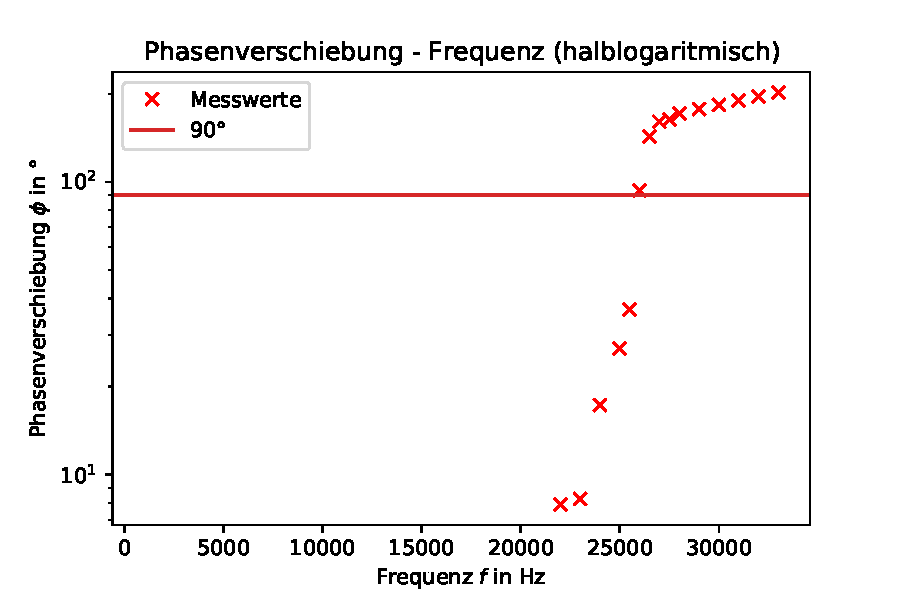
\includegraphics{phasenverschiebung.pdf}
      \caption{Phasenverschiebung in Abhängigkeit der Frequenz.}
      \label{fig:phasenverschiebung}
    \end{figure}
    \begin{figure}
      \centering
      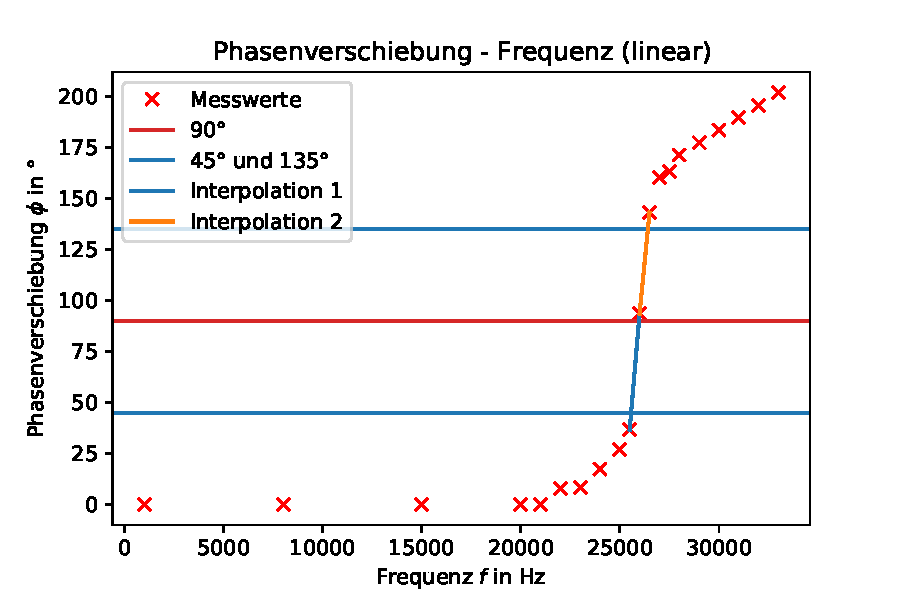
\includegraphics{phasenverschiebunglin.pdf}
      \caption{Phasenverschiebung in Abhängigkeit der Frequenz.}
      \label{fig:phasenverschiebung2}
    \end{figure}
    Die resultierenden Frequenzen lauten:
    \begin{center}
        $45°$$\rightarrow$$\omega_1=\SI[]{25.57}[]{kHz}$,\\
        $90°$$\rightarrow$$\omega_{res}=\SI[]{25.96}[]{kHz}$ und\\
        $135°$$\rightarrow$$\omega_2=\SI[]{26.41}[]{kHz}$.\\
    \end{center}
    Die theoretischen Werte lassen sich über die nachstehenden Gleichungen bestimmen.
    \begin{center}
        $\omega_{1,2}=\pm \frac{R}{2L}+\sqrt{\frac{R^2}{4L^2}+\frac{1}{LC}}$,\\
        $\omega_{res}=\sqrt{\frac{1}{LC}-\frac{R^2}{2L^2}}$
    \end{center}
  Damit folgt dann sofort:
  \begin{center}
      $45°$$\rightarrow$$\omega_1=(2.774\pm 0.011) \times 10^5\si[]{Hz}$,\\
      $90°$$\rightarrow$$\omega_{res}=(1.0398\pm 0.0027)\times 10^5\si[]{kHz}$ und\\
      $135°$$\rightarrow$$\omega_2=(1.175\pm 0.004)\times 10^5\si[]{kHz}$.\\
  
  \end{center}
  
  \begin{table}
    \centering
    \caption{Messdaten für die Resonanzüberhöhung und Phasenverschiebung}
    \label{tab:tab1}
    \begin{tabular}{c c c c}
      \toprule
      $f / \si{kHz}$ & $U_C / \si {\volt}$ & $U_0 / \si{\volt}$ & $\Delta t / \si{\micro\second}$\\
      \midrule
      1 & 18 & 37 & 0\\
      8 & 21 & 37 & 0\\
      15 & 28 & 37 & 0\\
      20 & 42 & 37 & 0\\
      21 & 50 & 37 & 0\\
      22 & 62 & 37 & 1.0\\
      23 & 80 & 36.5 & 1.0\\
      24 & 116 & 35 & 2.0\\
      25 & 200 & 35 & 3.0\\
      25,5 & 290 & 35 & 4,0\\
      26 & 340 & 32 & 10 \\
      26,5 & 260 & 30 & 15\\
      27 & 180 & 33 & 16.5\\
      27,5 & 140 & 34 & 16.5\\
      28 & 105 & 35 & 17\\
      29 & 80 & 35 & 17\\
      30 & 52 & 35 & 17\\
      31 & 44 & 35 & 17\\
      32 & 36 & 35 & 17\\
      33 & 32 & 35 & 17\\
      \bottomrule
    \end{tabular}
  \end{table}

  Die nach \autoref{eq:prozentuale} berechneten relativen Abweichungen betragen für $\omega_1$ 90.78\%, für 
  $\omega_2$ 77.9\% und für $\omega_{res}$ 74.59\%.
  Es wurden zudem einige Messwerte ausgelassen, da diese nicht signifikant zur Phasenverschiebung oder zur Resonanzüberhöhung
  beigetragen haben.
 
  
  \newpage
  \section{Diskussion}
  
  In diesem Versuch sollte zunächst in \autoref{sec:abklingdauer} die Abklingdauer bestimmt 
  werden. Das Ergebnis liegt hier bei $T_{ex} = 0.89\pm 0.08 \si[]{ms}$.
  Es liegen keine Vergleichswerte vor das Resultat scheint jedoch autentisch zu 
  sein.\\ Im nächsten Versuchsteil in \autoref{sec:apg} wurde dann der theoretische
  Widerstandswert des aperiodeischen Grenzfalls berechnet und festgestellt, das dieser
  um 31.2\% vom experimentell ermittelten Wert abweicht.\\ Im nächsten Kapitel
  \autoref{sec:res} wurde dann die Resonanzüberhöhung bzw. die Güte der Schaltung ermittelt.
  Der Experimentelle Wert liegt hier bei $155.1\pm 0.4$ und weicht damit um 182.5\% vom 
  errechneten Wert, welcher bei $q=45.63\pm 0.18$ liegt ab.\\ Im darauf folgenden 
  Abschnitt, \autoref{sec:phs} wurden dann die Frequenzen untersucht bei denen 
  die Phasenverschiebung bei 45°,90° und 135° liegt die hier gemessenen werte weichen für
  $\omega_1$ um 90.78\%, für $\omega_2$ um 77.9\% und für $\omega_{res}$ 74.59\% ab.\\\\ 
  Die großen Abweichungen bei allen Messwerten, werden vorallem daran liegen das 
  die Werte vom Oszilloskop nur ungenau abgelesen werden konnten und das diverse andere
  Faktoren wie Innenwiderstände vernachlässigt wurden.

  \newpage
  \section{Literaturverzeichnis}
  [1] TU Dortmund. V354: Gedämpfte und erzwungene Schwingungen. 2022.
\end{document}
